\begin{figure}[h]
    \centering
    \caption{Arquitetura de sistema da solução 1\_bertha após adaptação.}
    \begin{center}
        \begin{overprint}
            \onslide<1>\centering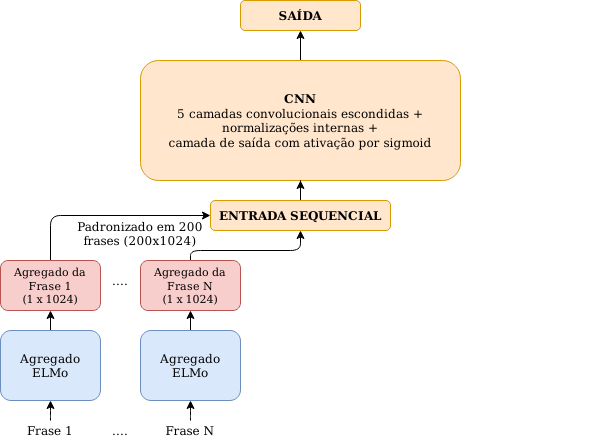
\includegraphics[width=0.50\textwidth]{img/1-bertha-arquitetura-sem-ri-corrigida.png}\onslide<2>\centering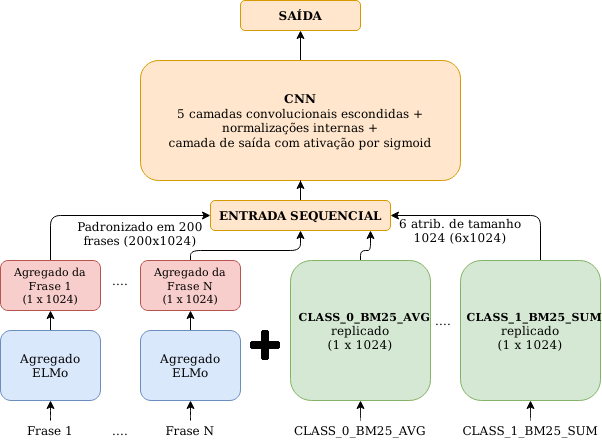
\includegraphics[width=0.50\textwidth]{img/1-bertha-arquitetura-com-ri-corrigida.png}
        \end{overprint}
    \end{center}
    \vspace{-0.0cm}
    \text{\footnotesize \textbf{Fonte:} O autor.}
    \label{fig:1-bertha-arquitetura-com-ri}
\end{figure}